%% LyX 2.1.0 created this file.  For more info, see http://www.lyx.org/.
%% Do not edit unless you really know what you are doing.
\documentclass[letterpaper,english,times]{speauth}
\usepackage[T1]{fontenc}
\usepackage[utf8]{inputenc}
\usepackage{array}
\usepackage{verbatim}
\usepackage{textcomp}
\usepackage{url}
\usepackage{graphicx}

\makeatletter

%%%%%%%%%%%%%%%%%%%%%%%%%%%%%% LyX specific LaTeX commands.
\pdfpageheight\paperheight
\pdfpagewidth\paperwidth

%% Because html converters don't know tabularnewline
\providecommand{\tabularnewline}{\\}

%%%%%%%%%%%%%%%%%%%%%%%%%%%%%% Textclass specific LaTeX commands.
\newcommand{\lyxaddress}[1]{
\par {\raggedright #1
\vspace{1.4em}
\noindent\par}
}

\makeatother

\usepackage{babel}
\begin{document}

\title{Understanding package management\\
through the lens of programming languages}


\author{Hisham~Muhammad\affil{1}, Lucas~Correia~Villa~Real\affil{2}
and Michael~Homer\affil{3}}


\address{\affilnum{1}PUC-Rio - Rio de Janeiro, Brazil\break\affilnum{2}IBM
Research - São Paulo, Brazil\break\affilnum{3}Victoria University
of Wellington - Wellington, New Zealand}
\begin{abstract}
Package management is instrumental for programming languages, operating
systems and system administration, and yet it is neglected by all
three areas as an implementation detail. For this reason, package
management lacks the same kind of conceptual organization present
in other disciplines. Moreover, we lack terminology to classify them
or to reason about their design trade-offs or issues that affect families
of similar managers. The multitude of package managers in modern systems
should be embraced, so we could start reasoning about them the way
we do about ecosystems of programming languages. In this paper, we
look at package management systems through this lens, sharing our
experience writing package managers for both a Linux distribution
and a scripting language. We categorize families of package managers
and discuss their design implications beyond particular implementations.
We also identify possibilities in the still largely unexplored area
of package manager interoperability.
\end{abstract}

\keywords{\noindent package management, operating systems, module systems,
filesystem hierarchy}

\maketitle

\section{Introduction}

Package management is an area that lies somewhere in the border between
programming languages, operating systems and system administration.
For this reason, it seems to be overlooked by all three fields as
an implementation issue. In the meantime, package management keeps
growing in complexity. New languages, new deployment models and new
portability requirements, all give rise to new package management
systems. Further, this is not simply a matter of competing implementations:
modern complex environments often require several package managers
to be used in tandem.

For example, when writing JavaScript web applications on a Mac environment,
a developer may require using Bower \cite{bower}, a package manager
for client-side JavaScript components. Bower is installed using \texttt{npm}
\cite{npm}, a package manager for \texttt{node.js} \cite{nodejs},
a JavaScript environment. On a Mac system, the typical way to install
command-line tools such as \texttt{npm} is via either Homebrew \cite{homebrew}
or MacPorts \cite{macports}, the two most popular general-purpose
package managers for Mac OSX. This is not a deliberately contrived
example; it is the regular way to install development modules for
a popular language in a modern platform.

In \cite{Burns2012Deploying} we have another example of a typical
software stack, where a deployment and management scenario for Ruby
on Rails applications is described combining a number of tools. It
uses Vagrant \cite{Hashimoto2013Vagrant} for virtual machine management;
Puppet \cite{Arrundel2011Puppet} for editing system configuration
files and driving the system-wide package manager on servers; Capistrano
for deploying the Ruby on Rails application, including installing
Ruby scripts and migrating database tables, driving RubyGems, the
language-specific package manager for Ruby modules (with Bundler to
mitigate module version conflicts); and RVM for managing conflicting
versions of Ruby itself. It is interesting to note the number of different
tools being used on top of each other to manage containment and compatibility
issues on various layers; and again, this is a typical, realistic
scenario.

The combinations of package managers change as we move to a different
operating system or use a different language. Learning one's way through
a new language or system, nowadays, includes learning one or more
packaging environments. As a developer of modules, this includes not
only using package managers but also learning to deploy code using
them, which includes syntaxes for package specification formats, dependency
and versioning rules and deployment conventions. Simply ignoring these
environments and managing modules and dependencies by hand is tempting,
but the complexity of heterogeneous environments and keeping track
of dependency updates can become burdensome — all these package managers
were created to solve pratical problems which the developer would
have to otherwise directly handle, after all. Another alternative
that is often proposed, especially by users of operating systems that
feature a system-provided package manager (as is the case of most
Linux distributions), is to avoid using multiple package managers
and use a single general-purpose package manager. This is, of course,
as much as a solution as trying to make everyone agree on a single
programming language, and this is the first of various analogies between
package management and programming languages that we will make throughout
this paper. The result is that the ecosystem is not getting any simpler,
and at first glance it seems that package management is indeed a largely
unsolved problem.

However, maybe the statement ``package management is an unsolved
problem'' simply does not make sense, and is akin to saying that
``programming languages are an unsolved problem''. In the programming
languages world we accept that the multitude of languages is a given.
Beyond that, we understand that there are families of languages with
different paradigms, with well-known tradeoffs. We also accept that
there is room for domain-specific languages (DSLs) and for general-purpose
languages. Most importantly, we know how to set boundaries for each
language and how to make DSLs and general-purpose languages interact.

We argue that all of these observations can be made with regard to
package management as well. In this paper, we discuss how these observations
map from the world of programming languages to that of package managers.
Most existing package management systems, however, are still oblivious
to the fact that they exist as part of a larger ecosystem, with parts
of it handled by other package managers. By discussing how programming
languages deal with these issues, we point to directions on how package
managers could follow their example, drawing on our experiences developing
both a system-wide package manager \cite{Muhammad2002WSL,Homer2010LCA}
and a language-specific package manager \cite{Muhammad2013LuaRocks}. 


\section{Paradigms of package management: filesystem-oriented vs. database-oriented}

It is customary to organize the landscape of programming languages
into paradigms, such as imperative, functional, object-oriented, and
so on. These paradigms describe the core conceptual frameworks on
top of which languages are designed. The paradigms a language is categorized
into inform users about particular design choices, and with these
choices come design trade-offs. Many of these trade-offs have been
studied and are well understood. A notable example is the Expression
Problem \cite{Wadler1998EP,Krishnamurthi:1998:SOF:646155.679709},
which poses a trade-off between traditional functional and object-oriented
approaches when extending code via separate compilation units: in
functional programming, it is easy to add new operations to a data
type (adding new functions), but it is not possible to extend the
type (adding new cases to the algebraic data type) without editing
the original code; in OOP, it is easy to extend the type (adding a
subclass), but it is not possible to add new operations to an existing
type (adding new methods to the original class) without editing code.
Once this trade-off is understood, it becomes easier to propose solutions
to mitigate it, such as open classes \cite{Clifton:2000:MMO:353171.353181}
and mixins \cite{Flatt:1998:CM:268946.268961}.

In the world of package managers, we can also identify general paradigms,
by looking at their core concepts and design trade-offs. Package managers
are programs that map relations between files and packages (which
correspond to sets of files), and between packages (dependencies),
allowing users to perform maintainance of their systems in terms of
packages rather than at the level of individual files. The central
design choice in a package manager, therefore, is how to perform those
mappings.

There are two approaches on how to map files to packages: the mapping
can be either \emph{internal} or \emph{external} to the hierarchical
structure of directories where the files reside. As this choice embodies
a series of trade-offs and is the single decision that affects the
design and implementation of a package manager the most, we identify
these as two paradigms of package management. When the mapping is
internal to the file hierarchy structure, we say that package management
is \emph{filesystem-oriented}. When it is external to the hierarchy
of files being managed, the mapping needs to be stored elsewhere:
on a database, or an equivalent structure that acts as one. We say
in these cases that management is \emph{database-oriented}. Most package
managers for Linux distributions, such as RPM and dpkg/APT, are database-oriented.
Filesystem-oriented package management is more often seen in language-specific
package managers, such as npm and Bower, but as we discuss in Section
\ref{sub:GoboLinux}, it can be performed system-wide.

Being database-oriented does not imply an opaque, binary database
format. LuaRocks 2.x uses a set of Lua tables (in \texttt{.lua} source
format) as its database. ArchLinux keeps its database as a tree under
\texttt{/var/lib/pacman/local}, with one subdirectory per package,
containing text files that list which files belong to which package,
as well as other metadata. The tree of Makefiles in BSD ports, containing
\texttt{install} and \texttt{uninstall} rules which control the mapping
of files to packages, can be considered a central database for package
management as well.

\begin{figure*}[t]
\begin{centering}

\includegraphics[scale=0.8]{python_pip}
\par\end{centering}

\begin{centering}
(a) Database-oriented management of Python modules. Modules for all
packages are stored together under \texttt{/usr/lib/python2.7/site-packages/}.\\
~
\par\end{centering}

\begin{centering}
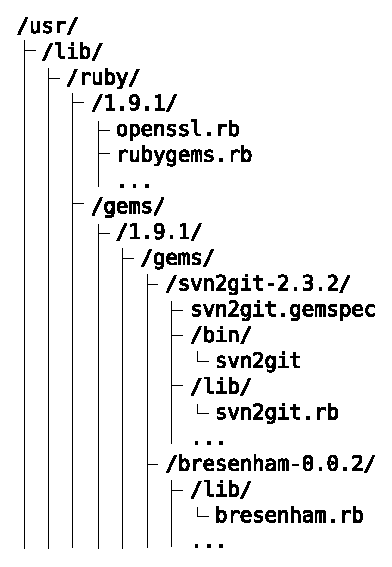
\includegraphics[scale=0.8]{ruby_rubygems}
\par\end{centering}

\begin{centering}
(b) Ruby modules managed with RubyGems. Each package gets its own
subdirectory under \texttt{/usr/lib/ruby/gems/1.9.1/gems/}.\\
~
\par\end{centering}

\protect\caption{\label{fig:Comparison-of-db-and-fs}Comparison of database-oriented
and filesystem-oriented package management styles.}
\end{figure*}


Figure \ref{fig:Comparison-of-db-and-fs} illustrates the two different
styles of package management. Figure \ref{fig:Comparison-of-db-and-fs}(a)
is representative of the database-oriented style. It shows the directory
structure using \texttt{pip}, the package manager for Python modules.
Note that all installed modules are stored under \texttt{/usr/lib/python2.7/site-packages/},
which was the default directory for locally-installed modules prior
to the introduction of \texttt{pip}. Database-oriented designs are
often chosen when the package manager needs to accomodate a pre-existing
directory structure. Conflicts are avoided through the use of the
Python module namespace, but may still occur in case of module clashes.
In this example, Pillow is a fork of the PIL (Python Imaging Library)
package, and reuses the same namespace. Both cannot be installed at
the same time. Figure \ref{fig:Comparison-of-db-and-fs}(b) showcases
the filesystem-oriented style, presenting the directory structure
produced by RubyGems, the package manager for Ruby. Each package has
its own subtree under a versioned directory, containing a Unix substructure
with \texttt{bin/}, \texttt{lib/} and so on. The \texttt{rubygems.rb}
module, part of the default installation of Ruby, takes care of finding
the appropriate files when modules are loaded with the \texttt{require}
function. Figure \ref{fig:pm-taxonomy} lists more examples and their
classification.

Initially it may seem that this is an implementation detail, and
that this distinction is, or should be, transparent to users of package
managers. As long as they can type a command to install a package
and then launch the program or load the library, how the manager keeps
its consistency is irrelevant. While this is true for end-users installing
packages and using applications and libraries, it is not true for
another category of users of package managers: those who do the packaging
of programs. In other words, this is akin to saying that on one hand
end-users of applications shouldn't care what language they are written
in, but on the other hand the language paradigm affects those who
write programs greatly.

The major trade-off between the filesystem-oriented and the database-oriented
approaches is whether applications should be aware of the file structure
defined by the manager or whether the manager should adapt to the
file structure defined by applications. This affects how the manager
tracks the mapping of files and how applications find their resource
files. 

In filesystem-oriented managers the mapping of files to packages is
simple. File conflicts are naturally avoided by storing files of different
packages in separate subtrees. Versioning conflicts between variants
of the same package can also be handled via the tree structure. The
structure also becomes more transparent to users, which can simplify
their experience. The run-time lookup of files by applications, however,
can be complicated, if they are oblivious to the structure defined
by the package manager. Applications must either agree beforehand
to this structure (which might be an option in domain-specific environments),
or the package manager has to do extra work to configure them to use
the structure; in the worst case, patching them.

Conversely, in database-oriented managers the mapping of files to
packages is more complicated. Applications may install files wherever
they please, and the package manager needs to keep track. This includes
handling potential conflicts if two packages want to use the same
pathname. Database-oriented systems will usually report on these conflicts
and forbid them. It is up to the integrator (such as a distribution
developer) who is building packages to resolve the conflict somehow.
Also, the package manager needs to verify that the database and the
contents of the filesystem remain in sync, which is trivial in the
filesystem-oriented approach. The run-time lookup of files on database-oriented
systems, on its turn, is greatly simplified. In most cases it will
be a non-issue, since each file is in the location the application
expected it to be in the first place. However, it does become an issue
when the file has been relocated by the integrator who built the package,
perhaps for solving conflicts.



Repository maintainers of database-oriented package managers often
solve versioning conflicts by resorting to filesystem-oriented approaches.
For example, the maintainer of Debian packages for the Lua virtual
machine patches its Makefile to install C headers under versioned
directories such as \texttt{/usr/include/lua5.3}, to avoid conflicts
of simultaneous Lua versions in the system installing \texttt{lua.h}.
Such changes propagate to users of these packages: Lua-based software
such as LuaRocks \cite{Muhammad2013LuaRocks} and Prosody \cite{prosody}
include code in their installation scripts specifically to handle
Debian locations. Meanwhile, FreeBSD uses \texttt{/usr/include/lua53}
and NetBSD uses \texttt{/usr/include/lua-5.3}. To reduce this kind
of incompatibility among downstream distributors, many upstream maintainers
adopt hierarchical versioning structures themselves: C headers for
Python, for example, install into versioned directories such as \texttt{/usr/include/python2.7}
by default in every system. It is unclear, however, which packages
are the ones where users will desire to keep simultaneously installed
versions and which are not; one might ask why \emph{all} C headers
aren't installed in a versioned way. In fact, when we look at Unix
shared libraries, we see that this is the case: the standard practice
is to install libraries in versioned files such as \texttt{libfoo.so.1},
with a \texttt{libfoo.so} symbolic link for user convenience. Note
that, as typical of filesystem-oriented approaches, there needs to
be some cooperation for run-time lookup, and indeed the dynamic linker
is aware of this structure and makes use of versioned filenames.



Filesystem-oriented managers also present their own set of challenges,
as the description of packages as set of files does not present a
full picture. Packages, especially in system-wide installations, often
need to perform global changes to the system, such as adding users
and setting environment variables. Some applications also include
database-oriented portions which are assumed to be updated by installation
scripts, such as the icon cache for the GTK+ widget library: any package
that installs new icons has to refresh this global cache. Non-relocatable
packages often assume hardcoded default paths in which resource files
are expected to be found; if the package manager employs a different
organization, it needs to reconfigure applications to make sure the
required files are found. One common solution is to use environment
variables, since applications often support setting custom paths via
variables in addition to the system-wide defaults. Most applications
can be installed in custom locations, with the installation prefix
being adjustable at compile time. The \texttt{/opt} directory is a
traditional location for filesystem-oriented organization of additional
packages. Core system services are often harder to relocate.

To use the filesystem or a database is a frequent design dilemma beyond
package management, especially on Unix systems, where ``everything
is a file'' is a long-standing tradition. Different styles of bootscripts
on Unix employ one or the other approach, with System V being the
archetypical file-hierarchy-based init system and BSD init using \texttt{/etc/rc.conf}
as a central configuration file. Program configuration can either
use on separate text-based configuration files under \texttt{/etc}
or a central registry of settings, such as GConf \cite{Pennington2002GConf}. 

In modern Linux distributions, the package manager is the most central
component for organizing the operating system. Database-oriented solutions
often are considered un-Unix-like (GConf, for instance, raises comparisons
to the Windows Registry \cite{Wallen2003GConfWin}). It is remarkable
that, in spite of the Unix philosophy, most Linux package managers
are primarily database-oriented.

\begin{figure*}[t]
\begin{centering}
\begin{tabular}{|c|c|c|}
\cline{2-3} 
\multicolumn{1}{c|}{} & {\footnotesize{}Filesystem-oriented} & {\footnotesize{}Database-oriented}\tabularnewline
\hline 
{\footnotesize{}Language-agnostic} & {\footnotesize{}}%
\begin{tabular}{c}
{\footnotesize{}Homebrew (Mac OS X)}\tabularnewline
{\footnotesize{}Nix}\tabularnewline
{\footnotesize{}PBI 8 (PC-BSD)}\tabularnewline
{\footnotesize{}GoboLinux}\tabularnewline
\end{tabular} & {\footnotesize{}}%
\begin{tabular}{c}
{\footnotesize{}RPM (RedHat/Fedora/etc.)}\tabularnewline
{\footnotesize{}dpkg/apt (Debian/Ubuntu/etc.)}\tabularnewline
{\footnotesize{}PBI 9 (PC-BSD)}\tabularnewline
{\footnotesize{}Pacman (ArchLinux)}\tabularnewline
\end{tabular}\tabularnewline
\hline 
{\footnotesize{}Language-specific} & {\footnotesize{}}%
\begin{tabular}{c}
{\footnotesize{}npm (server-side JavaScript)}\tabularnewline
{\footnotesize{}Bower (client-side JavaScript)}\tabularnewline
{\footnotesize{}RubyGems (Ruby)}\tabularnewline
{\footnotesize{}Cargo (Rust)}\tabularnewline
{\footnotesize{}LuaRocks 1.x (Lua)}\tabularnewline
\end{tabular} & {\footnotesize{}}%
\begin{tabular}{c}
{\footnotesize{}Cabal (Haskell)}\tabularnewline
{\footnotesize{}pip (Python)}\tabularnewline
{\footnotesize{}LuaRocks 2.x (Lua)}\tabularnewline
\end{tabular}\tabularnewline
\hline 
\end{tabular}
\par\end{centering}

\protect\caption{\label{fig:pm-taxonomy}A package manager taxonomy, with representative
examples}
\end{figure*}



\subsection{GoboLinux\label{sub:GoboLinux}}

GoboLinux \cite{Muhammad2002WSL} is a Linux distribution based on
the concept of installing each package in a separate installation
prefix. It was the first Linux distribution to be entirely based on
a filesystem-oriented approach to package management. Each program
is installed under its own versioned directory, such as \texttt{/Programs/Bash/4.3.28}
and \texttt{/Programs/GTK+/3.16.0}. This direct mapping of the package
structure to the directory layout allows one to inspect the system
using standard Unix commands. For example, to get a list of installed
packages, one only needs to issue \texttt{ls /Programs}.

As well as the individual program trees, a tree of symbolic links
also exists created collecting references to the files of every program
in the system together. A single directory contains symlinks matching
the structure of the ``\texttt{lib}'' directory of every program,
paralleling the contents of \texttt{/usr/lib} in a conventional layout.
In this way only a single entry in PATH is needed to find every executable
and libraries can be loaded using the ordinary linker mechanisms without
further configuration. An additional layer of fixed symlinks provides
backwards compatibility with the conventional Filesystem Hierarchy
Standard\cite{fhs}.

Since packages become self-described through the GoboLinux filesystem
hierarchy, the distribution features its own set of system management
tools built around scripting languages. At first, these scripts automated
tasks such as the installation of new packages (simply compressed
tar archives) and their ``activation'' in the system (namely, the
creation of symbolic links to their libraries, headers, executables,
and manuals) as well as their removal (achieved by deleting their
directory and the now-broken symbolic links). Over time, these scripts
inevitably became more complex as they were integrated with other
system tools and served as the pillars for \emph{Compile}, GoboLinux's
build system.

Taking inspiration from Gentoo's Portage system (which was itself
inspired from BSD Ports) \cite{Thiruvathukal2004Gentoo}, Compile
makes use of recipes that describe how to fetch the source code of
a piece of software and the sequence of commands required to build
and install it. Because recipes are frequently hand-written, it is
essential to make them as simple as possible so that users are encouraged
to contribute to the distribution's ecosystem. The approach adopted
by Compile is to embed as much code as possible in its build systems'
backends (e.g. Autoconf, Makefile, xmkmf, CMake), allowing the majority
of recipes to be described with little more than a couple of lines.
More complex build cases can be described by extending recipes with
regular shell scripting. Compile can also enable the installation
of packages through third-party package managers. More details of
that feature are given in Section \ref{sub:GoboLinux-Aliens}.

Up to GoboLinux 014.01, packages built with Compile had their prefixes
set to their versioned directory during their compilation. That had
a consequence in a considerable extent of software that use their
prefix directory for run-time lookups of \textit{shared }files (i.e.
those under\texttt{ /usr/share}) and impacted the layout of the GoboLinux
directory tree and its management scripts. Each versioned directory
received a \texttt{Shared} sub-directory containing that package´s
own files and a symbolic link named \texttt{share p}ointing back to
\texttt{/System/Links/Shared} (which managed links to the files of
each package's \texttt{Shared} directory), leading to code growth
and a deviation to the distribution's original design. As the Linux
userland ecosystem evolved, some new packages started to share files
through \texttt{/usr/lib\{64\}}, too. It is easy to picture how complicated
the task of a modern package manager can be nowadays, as even subtle
changes to filesystem namespace semantics can have profound impact
on the organization of this class of software. In GoboLinux, we fixed
this problem once and for all by introducing major changes to the
system's directory layout and by using a new compilation prefix \texttt{/System/Index}
common to all packages (Figure \ref{fig:gobofs}). Through this structure,
even though packages are organized in self-contained directories under
\texttt{/Programs}, applications can find their files through the
traditional Unix hierarchy, as \texttt{/usr} is a symbolic link to
\texttt{/System/Index}. 

\begin{figure*}[t]
\begin{centering}

\includegraphics[scale=0.8]{gobo_systemindex}
\par\end{centering}

\begin{centering}
(a) The filesystem is indexed with the use of directories and symbolic
links.\\
~
\par\end{centering}

\begin{centering}
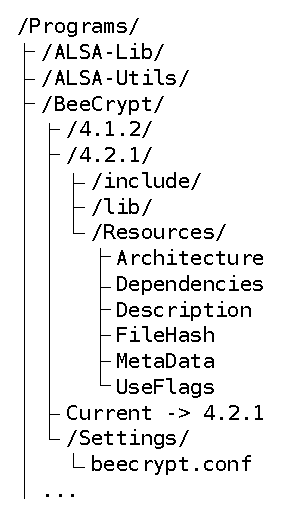
\includegraphics[scale=0.8]{gobo_programs}
\par\end{centering}

\begin{centering}
(b) Packages are managed through a versioned directory tree.\\
~
\par\end{centering}

\protect\caption{\label{fig:gobofs}GoboLinux file system hierarchy}
\end{figure*}


\begin{comment}
The mostly declarative style of GoboLinux recipes proved to be a success
among users and gave us greater freedom when modifying the build process.
We made major changes to the system's directory layout between releases
014 and 015 of the distribution, and the use of high-level descriptions
and our cautious avoidance of hardcoded paths allowed us to reuse
the majority of recipes with no changes.
\end{comment}


\begin{comment}
\begin{itemize}
\item parts of the Unix FS hierarchy which assume a single directory: /usr/share/icons

\begin{itemize}
\item effect this had on share/ in Gobo

\begin{itemize}
\item having to symlink /P/Foo/x.y/share into /S/L/share
\item launching helper indexing such as gtk-update-icon-cache upon each
installation 
\end{itemize}
\end{itemize}
\item discuss symlinks

\begin{itemize}
\item The ``virtualized'' Unix directories of GoboLinux avoid some compatibility
issues that affect other distributions: all executables appear at
the same time in /bin, /sbin, /usr/bin and so on.
\end{itemize}
\item the build system, the tooling for generating packages, is the central
piece of a package management system.

\begin{itemize}
\item not clear at first, but looking at package management systems they
all integrate the build process. Why?
\end{itemize}
\item Discuss the challenges of GoboLinux through the prism of its build
system (?)

\begin{itemize}
\item Tried to make it easy for users to build packages.
\item Took inspiration from systems such as Gentoo, which was itself inspired
from BSD Ports.
\item aim was to make the simple cases super-simple (like a 3-line script)
and the complex cases possible (leveraging the generality of shell
scripts)
\item This worked up to a point. Eventually, started requiring more and
more metadata, even for the so-called simple cases.
\item Further, this metadata had to be integrated with the deployed system. 
\item The ArchLinux build system seems to be a modern-day successor of this
style of build system in the Linux space.
\end{itemize}
\item tie in with the discussion of above section about includes? Gobo
pre-/S/I didn't need versioned includes when applications detect the
install prefix of libraries they depended on (e.g. via pkgconfig);
with /S/I, pkgconfig will return includedir as /usr/include, so this
becomes an issue: the recipe needs to point the conflicting program
to /P/Foo/x.y/include, or the user needs to temporarily symlink the
desired version (which is more fragile).

\begin{itemize}
\item Still, the compatibility gains for maintenance greatly outweigh the
losses, of course.\end{itemize}
\end{itemize}
\end{comment}



\subsection{Other filesystem-oriented approaches}

One of the earliest filesystem-oriented package managers to note is
GNU Stow \cite{stow}, which inherited ideas from Carnegie Mellon's
Depot \cite{Colyer1992Depot}. Stow focuses on the management of programs
installed on non-regular paths (e.g. on some user's home directory,
on external devices, etc). Given the path to one such program tree,
Stow ``activates'' it on the system by creating symbolic links to
the program's contents at a central location such as \texttt{/usr/local}.
Existing symbolic links are expanded with directories to manage conflicts.
A similar approach is taken by Encap \cite{encap}: packages are installed
onto a \texttt{/usr/local/encap/packageName-packageVersion} hierarchy,
with the management of symbolic links performed by the \texttt{epkg}
script. Unlike Stow, Encap is able to revert to a previous version
of a given package thanks to the directory names used at \texttt{/usr/local/encap}. 

The popularization of union-based filesystems brought novel ideas
into package management. The GNU Hurd community proposes the use of
GNU Guix to have packages installed in their own directories. Through
the use of user \textit{profiles}, then, union-mounts provided by
Hurd's \texttt{stowfs} will create a traditional Unix directory structure
view formed from all the files in the individual package directories
listed in that profile \cite{hurd}. The Push Button Installer (PBI)
of the FreeBSD-based PC-BSD distribution used for a long time a similar
structure to GoboLinux's \texttt{/Programs}. Packages managed by PBI
were installed on \texttt{/usr/Programs} and activated by symbolic
links at \texttt{/usr/local}. The fundamental difference between the
two is that, in PBI, package dependencies (i.e. a collection of shared
objects) are shipped along with the package. For instance, the Xpdf
package ships both with the \texttt{xpdf} executable as well as with
the Xorg libraries it depends on. The storage space taken by the many
duplicated files found across different packages is managed by PBI
through a simple deduplication method based on hardlinks \cite{pbi}.
Starting with the PC-BSD 10 series, the PC-BSD project revamped their
implementation of the PBI runtime containers so that they could benefit
from a virtualized \texttt{/usr/local} namespace. At the present time
that is still an ongoing work.

One last class of virtualization arose motivated by the widespread
adoption of cloud computing and is represented by projects such as
Docker \cite{Merkel2014Docker}. Docker provides an abstraction layer
so that users can deploy their applications (together with their dependencies)
inside \textit{containers} that run with isolated resources, as if
they were in a virtual machine. Linux kernel namespace and control
groups (cgroups) subsystems are used to implement Docker's fine-grained
control over the hardware and operating system resources. The container
environment can then contain only the necessary packages for a single
application, circumventing dependency chain conflicts that might arise
from installing multiple applications sharing a single filesystem
hierarchy. These technologies are giving birth to a new concept of
package management, as users no longer run into library versioning
conflicts between the various packages installed on their system:
they simply deploy conflicting packages as separate containers. Still,
this only shifts the problem to a larger granularity: the containers
themselves need to be managed, and various services communicating
with each other in separate containers will also have versioning compatibility
requirements.

\begin{comment}
\begin{itemize}
\item Short history of alternative approaches:

\begin{itemize}
\item earliest related work: GNU stow, encap. (Our paper from Workshop em
Software Livre mentions that, but we didn't really know about them
when making Gobo)
\item djb's /package structure
\item Zero Install (still active), Autopackage (dormant, ``packages must
be relocatable''), 
\end{itemize}
\item app dirs: RiscOS, Mac OSX. (Android and iOS?)
\item The Nix project has been around almost as long as GoboLinux. NixOS
is nowadays a serious contender in the world of server-oriented operating
systems.

\begin{itemize}
\item virtual machines: minimalism is making its way back in OS layout design.
(There have always been minimalistic Linux distributions, back from
the ``rescue'' distros such as Damn Small Linux and tomsrtbt (which
would fit in a floppy!).

\begin{itemize}
\item CoreOS, based on Gentoo, is the current representative of the minimalistic
server-oriented distro world.
\item Ubuntu Core was recently announced, and this might be a beginning
of a general trend of ``core'' OSes.

\begin{itemize}
\item Ubuntu Core ``snappy'' packages strongly resemble GoboLinux!
\end{itemize}
\end{itemize}
\item Homebrew, a package manager for Mac OS X, is a successful realization
of this idea. One of its original design criteria was to do package
management ``the GoboLinux way'' {[}in the git history of homebrew's
README.md we find them citing gobolinux{]} (so I guess that's the
most widespread legacy of our work)
\end{itemize}
\item What do we mean by filesystem facilities: a more powerful fs would
make things better?

\begin{itemize}
\item Back in 200x we mentioned {[}the ``clueless'' whitepaper{]} how
we needed more low-level tooling from the underlying operating system
in order to be able to realize some of the ideas of GoboLinux cleanly.
We were asking for more abstraction and isolation in userspace: essentially
we wanted union filesystems and possibly some sort of containers for
finer-grained isolation. Lacking those, we had to make do with chroot.
\item For a while we hoped that as underlying technology matured, these
ideas could come to fruition.
\item Docker seems to be proof of that; a container-based system that greatly
simplified application deployment.
\item However, Glauber Costa, one of the developers of the Linux Containers
system, described the limitations of that approach exposed the hackery
involved {[}did he write about it somewhere?{]}. Costa himself moved
away from containers and joined the efforts of the OSv project, a
minimalistic operating system targeting hypervisor-based architectures.\end{itemize}
\end{itemize}
\end{comment}



\section{Language-specific vs. language-agnostic package managers}

\begin{figure*}[t]
\begin{centering}
{\footnotesize{}}%
\begin{tabular}{|c|>{\centering}p{0.1\paperwidth}|>{\centering}p{0.1\paperwidth}|>{\centering}p{0.1\paperwidth}|>{\centering}p{0.1\paperwidth}|}
\cline{2-5} 
\multicolumn{1}{c|}{} & \multicolumn{4}{c|}{{\footnotesize{}Language-specific managers}}\tabularnewline
\hline 
{\footnotesize{}Package managers} & \textbf{\footnotesize{}npm} & \textbf{\footnotesize{}RubyGems} & \textbf{\footnotesize{}NuGet} & \textbf{\footnotesize{}LuaRocks}\tabularnewline
\hline 
\hline 
{\footnotesize{}Portability} & \multicolumn{4}{c|}{{\footnotesize{}OS-independent (all Unix, Windows)}}\tabularnewline
\hline 
{\footnotesize{}Installs code written in} & %
\begin{tabular}{c}
{\footnotesize{}JS family,}\tabularnewline
{\footnotesize{}C/C++}\tabularnewline
\end{tabular} & %
\begin{tabular}{c}
{\footnotesize{}Ruby, C/C++,}\tabularnewline
{\footnotesize{}JVM family}\tabularnewline
\end{tabular} & {\footnotesize{}any .NET, C++} & {\footnotesize{}Lua family, C/C++}\tabularnewline
\hline 
{\footnotesize{}Files managed} & %
\begin{tabular}{c}
{\footnotesize{}JS scripts,}\tabularnewline
{\footnotesize{}JS modules}\tabularnewline
\end{tabular} & %
\begin{tabular}{c}
{\footnotesize{}Ruby scripts,}\tabularnewline
{\footnotesize{}Ruby modules}\tabularnewline
\end{tabular} & %
\begin{tabular}{c}
{\footnotesize{}.NET and}\tabularnewline
{\footnotesize{}native packages}\tabularnewline
\end{tabular} & %
\begin{tabular}{c}
{\footnotesize{}Lua scripts,}\tabularnewline
{\footnotesize{}Lua modules}\tabularnewline
\end{tabular}\tabularnewline
\hline 
{\footnotesize{}Supports per-user install} & \multicolumn{4}{c|}{{\footnotesize{}yes}}\tabularnewline
\hline 
\multicolumn{1}{c}{} & \multicolumn{1}{>{\centering}p{0.1\paperwidth}}{} & \multicolumn{1}{>{\centering}p{0.1\paperwidth}}{} & \multicolumn{1}{>{\centering}p{0.1\paperwidth}}{} & \multicolumn{1}{>{\centering}p{0.1\paperwidth}}{}\tabularnewline
\end{tabular}
\par\end{centering}{\footnotesize \par}

\begin{centering}
{\footnotesize{}}%
\begin{tabular}{|c|>{\centering}p{0.1\paperwidth}|>{\centering}p{0.1\paperwidth}|>{\centering}p{0.1\paperwidth}|>{\centering}p{0.1\paperwidth}|}
\cline{2-5} 
\multicolumn{1}{c|}{} & \multicolumn{4}{c|}{{\footnotesize{}Language-agnostic managers}}\tabularnewline
\hline 
{\footnotesize{}Package managers} & \textbf{\footnotesize{}Nix} & \textbf{\footnotesize{}Homebrew} & \textbf{\footnotesize{}RPM} & \textbf{\footnotesize{}GoboLinux}\tabularnewline
\hline 
\hline 
{\footnotesize{}Portability} & {\footnotesize{}Linux/OSX} & {\footnotesize{}OSX} & {\footnotesize{}Linux/AIX} & {\footnotesize{}Linux/Cygwin/OSX}\tabularnewline
\hline 
{\footnotesize{}Installs code written in} & \multicolumn{4}{c|}{{\footnotesize{}any language}}\tabularnewline
\hline 
{\footnotesize{}Files managed} & \multicolumn{4}{c|}{{\footnotesize{}all kinds}}\tabularnewline
\hline 
{\footnotesize{}Supports per-user install} & {\footnotesize{}yes} & {\footnotesize{}no{*}} & {\footnotesize{}no} & {\footnotesize{}yes}\tabularnewline
\hline 
\multicolumn{5}{l}{{\footnotesize{}{*} different installation prefixes are supported
but }\texttt{\footnotesize{}/usr/local}{\footnotesize{} is strongly
recommended.}}\tabularnewline
\end{tabular}
\par\end{centering}{\footnotesize \par}

\protect\caption{\label{fig:langspec-vs-langagn}Contrasting language-specific and
language-agnostic package managers}
\end{figure*}


In the world of programming languages, there is a distinction between
DSLs and general purpose languages. Categorizing languages in one
camp or another is not always easy, but a working definition is that
domain-specific languages are those designed with a specific application
domain in mind, and general purpose languages are the complementary
set, that is, those languages designed not with a particular domain
in mind, but rather focusing on general areas such as ``systems programming''.

While we tend to see DSLs as smaller languages than their general-purpose
counterparts (and in fact early literature used to term them ``little
languages'' \cite{Bentley:1986:PPL:6424.315691}), what defines a
language as being a DSL is the \emph{inclusion} of features tailored
for a domain. This means that a domain-specific language may end up
including all features normally understood as those defining a general
purpose language. MATLAB, for instance, is a complete programming
language, but its wealth of features for numerical computing it is
often regarded as being domain-specific \cite{Gill:2014:DLC:2611429.2617811,Fowler2005LanguageWorkbench}.

In the world of package management, there is also a distinction between
domain-specific and general purpose systems, but it is better defined.
Language-specific managers are designed to be used in a particular
\emph{language ecosystem}. This ecosystem usually focuses around a
single language (hence the name ``language-specific''), but that
is not necessarily the case: environments such as .NET and the JVM
make this evident, but other languages also grow into families: for
example, LuaRocks was written for Lua but also supports MoonScript
and Typed Lua; npm supports JavaScript, CoffeeScript, TypeScript and
others. Besides, these VM-based ecosystems usually support loading
native extensions, and therefore they must also support building and
integrating libraries usually written in C or C++ (or, in the case
of RubyGems with JRuby, Java). A language-specific package manager,
therefore, is almost never specific to code written in a single language.
Like domain-specific programming languages which are not necessarily
much smaller than their general-purpose counterparts, the more sophisticated
language-specific package managers are in effect general package managers
with specific support for an ecosystem added. They need to build and
deploy executables, native libraries and resource files written in
different languages, keep track of installed files, check dependencies,
perform network operations and manage remote repositories. Some of
these tasks can be simplified due to ecosystem-specific assumptions,
but many are equivalent in complexity to the tasks of a system-wide
package manager.

This leads us to question why should we have language-specific managers
at all, if they replicate so much of the work done by general-purpose
package managers. Two arguments in defense of language-specific managers
are scalability and portability. If we compare the number of packages
provided by a typical Linux distribution versus the number of modules
available in mature module repositories from scripting languages,
it becomes clear that the approach of converting everything into native
packages is untenable: for example, while the repository for the Debian
Linux distribution features 43,000 packages in total, the Maven Central
repository for Java alone contains over 103,000 packages, with the
advantage that the repository is portable to various platforms, some
of which lacking a built-in universal package manager (Microsoft Windows
being a notable case). Still, this kind of effort duplication does
happen: the Debian repository contains 715 packages of Ruby modules;
this is a far cry from the 100,000 modules in the RubyGems repository.

Figure \ref{fig:langspec-vs-langagn} contrasts language-specific
and language-agnostic package managers, through a few examples. Language-specific
package managers tend to be highly portable, even if the modules in
their repositories are not. For example, while most packages for NuGet
are Windows-specific, the manager itself has been ported to Unix systems
via Mono; packages that do not depend on Windows APIs can be shared
by various platforms. Language-agnostic managers are generally system-specific,
and may present some degree of portability to other similar OSes.
Note that the extent of portability of all language-agnostic managers
in Figure \ref{fig:langspec-vs-langagn} is limited to specific Unix
variants. Those managers support packaging programs written in any
language and for that reason do not expect particular file formats
or subdirectory layouts. Language-specific managers make more assumptions
in that regard, and also support customizing the installation directory
prefix, which is a necessity for running as a non-privileged user.
Some system-wide managers, like Nix and GoboLinux support per-user
installations, but that often requires patching packages for removing
hardcoded pathnames. Homebrew supports this feature as a tool, but
their packages are not adapted for that, so per-user installations
are discouraged.


\subsection{LuaRocks}

LuaRocks \cite{Muhammad2013LuaRocks} is a package manager for the
Lua ecosystem. It was developed building on our previous experience
writing package management tools for GoboLinux and adapting them to
the realities of a language-specific manager.

The package specification format (\emph{rockspec}) was largely influenced
by GoboLinux, and LuaRocks pushes the use of declarative specifications
even further. While the \texttt{.rockspec} files themselves are actually
Lua scripts, LuaRocks loads them using a restricted execution environment
that disables the Lua standard libraries; they essentially consist
of variable declarations, describing the package via Lua tables (Lua's
single data structure, which combines numeric and associative arrays).



Another design feature inherited from GoboLinux was the support for
multiple build back-ends. In most language ecosystems, at any point
in time a single build tool is well-established as a standard (such
as \texttt{easy\_install} and later \texttt{pip} for Python, Rake
for Ruby, ExtUtils::MakeMaker and later Module::Build for Perl). In
the Lua world, by the time LuaRocks was conceived, in spite of several
contenders, there was no clear winner as a standard build tool. To
deal with the variety of build systems, OS-level package managers
typically let developers call their preferred build tools explicitly
in imperative scripts. LuaRocks attempted to solve this in a more
controlled manner, with a system of plugins for the various tools,
akin to the one used in GoboLinux. In LuaRocks, each plugin is implemented
as a Lua module, selected through an entry in the rockspec. For example,
using \texttt{build.type=\textquotedbl{}cmake\textquotedbl{}} causes
LuaRocks to invoke CMake with the appropriate arguments. We also included
a simple built-in build system, invoked via \texttt{build.type=\textquotedbl{}builtin\textquotedbl{}},
which is able to install Lua files and portably compile C code into
Lua modules. This proved a success among developers: at the time of
this writing, 75\% of all packages in the LuaRocks repository use
the built-in build system.



LuaRocks installs all packages into a sandbox directory and later
moves them to their final destinations. The actual installation prefix
is never informed to the build system under execution. This prevents
a package from hardcoding its own installation directory in its source
code. While the ability to do this is a feature sometimes requested
by developers (as it would make it easier to load asset files, for
example), disallowing hardcoded paths ensures that every package built
is relocatable. Having fully relocatable packages is rare on Unix,
but is an expected feature on Windows. Having to cater to such conflicting
requirements is a constant in writing portable software; to alleviate
the issue of finding asset files, one of the authors developed a Lua
module called \texttt{datafile} %
\footnote{\url{http://github.com/hishamhm/datafile}, also available via \texttt{luarocks
install datafile}%
}, which resolves directory locations portably at run-time.



As it also happened with GoboLinux, having a high-level description
format allowed us to make radical changes to the installation layout
once that proved necessary. Since LuaRocks does not provide to specification
files any knowledge of the final directory structure, this change
was even less impacting for users than the change on GoboLinux: all
existing rockspecs could be used in the new directory layout without
any changes. This level of information hiding, extending not only
the installation prefix, but to all subdirectories, was only possible
because we were dealing with a language-specific manager, where we
could make assumptions about the contents of files (Lua source code
and binary dynamic libraries) and how they would be later used (as
command-line scripts or loaded by Lua through its package loader system).





The design changes that LuaRocks underwent from version 1.0 to version
2.0 were due to lessons learned on the specificities of language-specific
package management. The original design of LuaRocks was filesystem-oriented,
like GoboLinux. Each version of an installed package was given its
own directory and each category of files got its own subdirectory.
For example, for module \texttt{lpeg 0.12-1} one would store Lua files
in \texttt{\$PREFIX/lib/luarocks/rocks/lpeg/0.12-1/lua}. LuaRocks
included then a custom wrapper for Lua's \texttt{require()} function
in module \texttt{luarocks.require}. Once this module was loaded (either
via plain \texttt{require()} or via a command-line flag), subsequent
calls to \texttt{require()} would match module names to file locations,
taking into account the dependency trees of previously loaded modules.
This allowed multiple versions of a module to coexist in an installation,
and let modules load the correct versions of their dependencies transparently.
The approach of loading a custom \texttt{require()} function is the
same as adopted by RubyGems. However, many Lua users perceived the
wrapper as tampering with a standard library function, and disliked
having to perform an initial setup in their scripts for using modules
installed via LuaRocks %
\footnote{Since Ruby 1.9, the interpreter preloads the \texttt{rubygems} module
automatically; in prior versions uses had to add \texttt{require 'rubygems'}
explicitly. This was never an option for Lua due to the language's
minimalistic design, rendering LuaRocks as a strictly optional component.%
}. For LuaRocks 2.0, the design was changed to be database-oriented,
so that Lua modules could be installed into a typical Unix-like layout
that matched the default configuration of the Lua interpreter's package
loader. Since now Lua modules from all packages were installed into
a single directory such as \texttt{\$PREFIX/share/lua/5.3}, a database
had to be put in place matching files to packages. We kept to Lua's
minimalistic approach, using a plain-text manifest file (loadable
as Lua code) as a database. Supporting multiple versions of the same
package installed at the same time is still possible, but requires
the now-optional custom package loader, which produces versioned filenames
such as \texttt{\$PREFIX/lib/5.3/lpeg-0.11-1.so} when the dependency
graph requires an old version of a module.


\section{Integration between languages vs. integration between package managers}

Programming languages, both general-purpose and domain-specific, frequently
have points of integration between each other, in the form of foreign
function interfaces (FFIs). Code written in one language can frequently
call into code written in another language, sometimes with some adapter
code in between. Domain-specific languages are in fact frequently
embedded in general-purpose languages and in programs.

The same is not true of general-purpose and domain-specific package
managers. Integration between two package managers is almost unheard
of, even when they may be found on the same system. Instead, a subset
of packages distributed through a domain-specific package manager
are repackaged in the format of the general-purpose system. These
packages are fully integrated with the broader system and fully detached
from the domain-specific manager. Packages that were not repackaged
are still available by using the domain-specific system, but others
are available twice, potentially in different versions and with different
configurations. Debian experimented with a \texttt{rubygems-integration}
package that provided a limited connection between APT and RubyGems,
allowing Debian packages of individual RubyGems to satisfy dependencies
in the gem tool, but encountered nontrivial complications in doing
so~\cite{debian-ruby-trouble,debian-ruby-packaging}. Debian has
not yet pursued even this level of integration for other widely-used
domain-specific package managers, and the integration it has for RubyGems
is ad-hoc and highly specialized. In Section~\ref{sub:GoboLinux-Aliens}
we discuss our attempt at deeper integration in GoboLinux, but we
are aware of no other such integrations beyond what Debian performs.

A weaker form of one-way integration between package managers occurs
when the system-wide manager uses the language-specific package manager
merely as a build system. An example is the use of LuaRocks by Buildroot
\cite{buildroot}. Buildroot is a system for compiling full-system
images for embedded environments, which has its own package specification
format. It uses LuaRocks as a build tool: the Buildroot specification
scripts launch LuaRocks to generate Lua modules and then collect and
integrate them to the system.


\subsection{GoboLinux Aliens\label{sub:GoboLinux-Aliens}}

In GoboLinux we researched the idea of building a foreign function
interface (FFI) of sorts into our general-purpose package manager,
which we called Aliens\cite{Homer2010LCA}. Aliens provides an API
to write shims that connect the general-purpose system package manager
with domain-specific package managers.

With Aliens, packages in the general-purpose manager may express a
dependency on a package provided by a supported domain-specific manager:
for example, a package that requires the Perl \texttt{XML::Parser}
module, available from CPAN, can express a dependency ``\texttt{CPAN:XML::Parser
>= 2.34}''. The Aliens system directs such a dependency to a translating
shim, which uses the CPAN tool to confirm whether it is satisfied,
to install the package (and its dependencies) if required, and to
upgrade it, communicating any necessary information back to the general-purpose
manager. The shim can then make symbolic links for any binaries or
native libraries that have been installed. Any package in one of the
supported domain-specific managers is automatically available in this
way, without creating wrapper packages.

The domain-specific managers themselves are not modified in this process.
Each system is given complete control of a directory tree, and the
relevant languages configured to search in that tree. This protects
against changes in the functioning of the third-party systems, and
allows users to access them directly as well. A drawback, however,
is that the domain-specific managers do not have reciprocal access
to the wider system: installing a RubyGem that depends on a native
library will not innately result in the native dependency being satisfied.
The cross-platform nature of these systems makes even specifying such
information in a machine-readable way difficult, although some, notably
LuaRocks, make the attempt.

Not all domain-specific package managers lend themselves to this integration.
Some are resistant to placing their files within a restricted directory
tree, preferring to install into the global filesystem hierarchy where
they may interfere with each other and the system, while others do
not mechanize well. This limited coverage is an additional drawback
of the Aliens approach, but one that is limited to failing to solve
an existing problem, rather than creating a new one. As with programming
languages, a consensus implementation platform would inevitably be
simpler, but social and technical factors make it impractical. FFIs,
and Aliens, attempt to bridge the gap, with reasonable success.


\section{Conclusion}

In this paper, we presented an analysis of the landscape of existing
methodologies for package management, substantiated by our practical
experiences in the development and maintenance over the years of a
system-wide package manager for a Linux distribution and a portable
package manager for a scripting language. Package management is an
area that is notably neglected in academic studies, but is one of
practical impact in the design of modern operating systems and module
systems for programming languages, and a central issue in system administration.
With this work, we provide the beginnings of a conceptual organization
of approaches for package management, an area that lacks even common
terminology, and where many of the same design issues are faced and
dealt with time and again.

In the realm of programming languages, the existing conceptual organization
is useful in various levels. As one learns about a new programming
language, one can immediately gather some insight about its workings
by learning whether it is imperative or functional, statically-typed
or dynamically-typed, if it features eager or lazy evaluation. One
is also able to reason generally about whole families of languages,
but studying design issues and trade-offs that apply to all of them. 

Similar methods of classification are needed for package managers.
By identifying families of filesystem-oriented and database-oriented
package managers, we were able to point out issues common to them
and the general solutions in use. It is notable how many of the package
managers we researched for this work went through similar changes,
and how many of their experiences match our own.

Package managers deal fundamentally with the mapping between the file-level
organization of the filesystem and the higher-level concept of packages.
We observed that filesystem-oriented designs are preferrable as they
tend to have less problems with conflict resolution, but they require
some level of control on how run-time lookup happens, to ensure that
it is consistent for all packages. We observe that this control exists
when language-specific package managers are bundled with the language
environment, as is the case with npm for node.js and RubyGems for
Ruby. These managers were free to adopt filesystem-oriented designs
since they adjusted their module loaders accordingly. The other way
to exert this control over run-time lookup is to employ a system-wide
lower-level solution as we did in GoboLinux with the \texttt{/System/Index}
tree of symbolic links or in the stowfs filesystem virtualization
proposed for GNU Hurd. Database-oriented designs, on the other hand,
are more generally applicable, but are more opaque to their users
and are more prone to package conflict and file-to-package synchronization
issues. For these reasons, we advocate filesystem-oriented systems
in general, but we also recognize that there are situations where
a database-oriented solution works best to preserve compatibility
with the ecosystem at play, as was the case with LuaRocks.

Our classification of package managers as language-agnostic and language-specific
highlighted the complementary qualities of these two classes of managers.
The existence of language-specific package managers distributes integration
efforts, as upstream module developers are often the package integrators
themselves. This allows scaling repositories way beyond what is possible
through the work of OS distribution maintainers, but also generates
some tension between the language and distribution communities as
perceived duplicate work and incompatibilites happen. Through our
experience in both ends of the spectrum of package management — from
low-level distribution management in GoboLinux to high-level language
modules in LuaRocks — we observed a necessity for these different
levels of system organization to recognize each other and aim for
cooperation. Package managers do not exist on their own, but are part
of an ecosystem in which other package managers often take part. We
shared our experience in progressing on this direction with the GoboLinux
Aliens project, and we plan to further pursue FFI-style package management
interoperability. Future directions for LuaRocks include a plug-in
system through which a closer integration with the host system may
be implemented.

New package managers will continue to appear, as new languages and
environments give rise to new needs. Since new languages and environments
invariably give rise to new package managers, it is important to take
this issue into account, understanding how they interact with the
filesystem organization and with run-time systems. Doing this from
early on keeps possibilities open for better designs that less prone
to ``dependency hell'' and versioning conflicts.

\begin{acks}
Gobo
\end{acks}
\renewcommand{\refname}{REFERENCES}

\bibliographystyle{wileyj}
\bibliography{gobo}

\end{document}
